\documentclass{article}%You can define the type of paper here.
%%Useful packages that I commonly use.
\usepackage[numbers]{natbib}%Bibliography package (help at http://merkel.zoneo.net/Latex/natbib.php).
\usepackage{url}%Package to highlight url.
\usepackage{times}%Sets font to be times.
\usepackage{alltt}%Allows the use of verbatim (good for printing out code).
\usepackage{graphicx}%Used to import images.
\usepackage{amsmath, amssymb, amscd, gensymb}%Contains the AMS expanded math symbols library.
%%For those who want smaller margins, you can use this:
\usepackage[top=1in, bottom=1in, left=1in, right=1in]{geometry}

\begin{document}

    %%Title
    \title{Simulation and Modeling\\Project II: Ice Column Temperatures}
    \author{Clinton McKay}
    \maketitle

    %%Makes the paper use two collums
    \twocolumn

    %%Introduction-------------------------------------------------------------------------------------
    \section{Introduction}
    Glaciers are a natural phenomena that exhibit the interesting property of being able to flow even
    though they consist of ice. 
    In this project we will investigate the transfer of energy through 
    one-dimensional section of a glacier. 
    In this case we will observe the temperature at different depths 
    subject to the internal forces, and geothermal energy released from the ground at the base of the 
    glacier. 

    %%Method------------------------------------------------------------------------------------------
    \section{Method}
    \subsection{System}
    The formula used to model the ice temperature was modeled using the following equation.
    \begin{align*}
           \frac{\partial \theta}{\partial t} &= \frac{k}{\rho C_p} \frac{\partial^2 \theta}{\partial z^2}
                                              -w(z) \frac{\partial \theta}{\partial z}
                                              -u(z) \frac{\partial \theta}{\partial x}
                                              +\frac{\phi(z)}{\rho C_p}
    \end{align*} 
    There are four main components to the equation. 
    The first component $\frac{k}{\rho C_p} \frac{\partial^2 \theta}{\partial z^2}$ models the diffusion of the temperature in the ice. 
    At a minimum, there will be a straight temperature gradient between the basal and the surface temperatures.

    The next piece, $w(z) \frac{\partial \theta}{\partial z}$ is the flow of the temperature in the ice. 
    Since, there is precipitation that accumulates at the surface of the ice, the ice will begin ``flowing'' down. 
    In effect, the temperature is transfered downwards towards the base of the ice. 
    The flow downwards is not consistent, instead it decreases with depth. Representing the vertical velocities is achieved with $w(z)$
    \begin{align*}
        w(z) &= (\dot{a} + u_s \frac{\partial z_s}{\partial x}) \sigma(z)
    \end{align*}
    The main variable of interest is $\dot{a}$, which represents the precipitation accumulation rate. 
    The other variables $u_s$ and $\frac{\partial z_s}{\partial x}$, represent the horizontal surface velocity and the surface slope of the ice. 
    The last variable $\sigma(z)$ returns a normalized set of depths in the glacier. 

    The third component $u(z) \frac{\partial \theta}{\partial x}$ represents transfer of heat caused by the horizontal flow of the glacier. 
    Since this model represents a one-dimensional system in the depth direction of the glacier, it forces this term to become static vector of velocities at increasing depths. 
    The decrease of horizontal velocity at the increase of depth is called the horizontal shear of the glacier. 

    Last, we have the source term $\frac{\phi(z)}{\rho C_p}$. 
    Like with the previous component, it is also a static representation of the heat generated from the deformation of the ice. 
    The heat generated increases with the depth as the pressure increases. 

    The partial differential equation may be able to simulate the ice, but there are a few false assumptions.   
    The first is that the ice does not flow at the base. 
    To restructure the formula to reflect this change, $u(z)$ becomes:
    \begin{align*}
        u(z) = u_b + 0.8(u_s - u_b)
    \end{align*}
    Where $u_s$ and $u_b$ represent the horizontal surface and basal velocities. 
    Next, we must be aware that any sliding object is going to produce heat as a byproduct of friction. 
    To account for this we need to incorporate an additional heat source at the base of the glacier.  
    \begin{align*}
        Q_f = \rho g (z_s - z_b) \frac{\partial z_s}{\partial z} u_b
    \end{align*}  
    Where $z_s$, $z_b$, $g$, $\rho$, and $\frac{\partial z_s}{\partial z}$ represent the surface elevation, base elevation, gravitational pull, ice density and the slope of the ice respectively. 

    \subsection{System Boundaries}
    The system consists of two boundaries. 
    For simplicity, the top of the glacier remains at a constant temperature throughout the year and the base of the glacier is heated by frictional forces. 
    There is still a heat source to consider, the geothermal heat flow $Q_{geo}$. 
    Heat flow is a form a diffusion, knowing this can assume that $k \frac{\partial \theta}{\partial z} |_{z=z_b}= Q_{geo}$ as long as $\theta_N$ is below $\theta_{PMP}$.

    \subsection{Objective}
    Using the equation to model the system. 
    The goal of this project is to find the optimal values for $\dot{a}$ and $u_b$ such that the sum squared error between the simulation temperatures and the actual data is minimized. 
    The simplex algorithm will be used to find the optimal values.  

    \subsection{Program}
    The program itself consists of two files.
    \begin{description}
        \item[main.py] Main execution script. 
        Calls all the necessary modules to find an optimal solution for $\dot{a}$ and $u_s$.
        \item[IceColumn.py] 
        \begin{description}
            \item[IceColumn] Contains all of the logic to run the simulation. 
            The diffusion matrix is calculated in the {\it diffusion\_matrix } method and the advection matrix is calculated in the {\it advection\_matrix} method. 
            \item[Icetimizer] Serves as a wrapper for the {\it scipy.optimize.fmin } function. 
        \end{description}
        \item[results.yml] Contains output from {\it scipy.optimize.fmin}. 
    \end{description}

    %%Verification------------------------------------------------------------------------------------
    \section{Verification of Program}
    To verify the accuracy of the simulation. 
    It was compared against an actual dataset consisting of temperature samples from a glacier. 
    The simplex algorithm was used to find an optimal $\dot{a}$ and $u_b$ such that the simulation fits closely to the real data. 

    Finding an optimal $\dot{a}$ and $u_b$ required 178 iterations of the {\it fmin} function (which exceeded the maximum allowed iterations). The minimum sum squared error found was $~5.50$ and this was achieved by setting $\dot{a} = 3.55x10^-3$ and $u_b = 3.49$. $ftol$ and $xtol$ for {\it fmin} were set to 0.001.

    %%Data--------------------------------------------------------------------------------------------
    \section{Data}
    The original data and data produced by the simulation can be found in Tables 1 \& 2. 
    \begin{table}[h!]
        \centering
        \begin{tabular}{c|c}
            $z$ (meters) & $\theta$ (C$\degree$)\\
            \hline
            -801. &  -1.4404231\\
            -741. &  -3.3368846\\
            -721. &  -4.3305769\\
            -701. &  -5.3550385\\
            -681. &  -6.4179615\\
            -661. &  -7.3731923\\
            -641. &  -8.3976538\\
            -621. &  -9.3298077\\
            -601. &  -9.9696538\\
            -581. & -10.947962 \\
            -561. & -11.572423 \\
            -541. & -12.012269 \\
            -521. & -12.652115 \\
            -501. & -12.630423 \\
            -481. & -12.654885 \\
            -461. & -13.817808 \\
            -441. & -13.834577 \\
            -421. & -12.9975   \\
            -401. & -13.429654 \\
            -381. & -13.261808 \\
            -361. & -13.863192 \\
            -341. & -13.472269 \\
            -321. & -13.565962 \\
            -301. & -13.782731 \\
            -281. & -13.168731 \\
            -261. & -13.131654 \\
            -241. & -12.963808 \\
            -221. & -12.095962 \\
            -201. & -12.0435   \\
            -181. & -12.152577 \\
            -161. & -11.577038 \\
            -141. & -11.3015   \\
            -121. & -11.279808 \\
            -101. & -10.5735   \\
             -81. & -10.074885 \\
             -61. &  -9.6993462\\
             -41. &  -9.5238077\\
             -21. &  -9.4867308\\
              -1. &  -9.6111923\\
        \end{tabular}
        \caption{The original dataset. Consists of temperature samples at 20 meter intervals. }
    \end{table}

    \begin{table}[h!]
        \centering
        \begin{tabular}{c|c}
            $z$ (meters) & $\theta$ (C$\degree$)\\
            \hline
            -801. & -3.68598881\\  
            -741. & -4.45282715\\
            -721. & -5.21291623\\
            -701. & -5.95959279\\
            -681. & -6.68643623\\
            -661. & -7.3873924 \\
            -641. & -8.05692103\\
            -621. & -8.69008464\\
            -601. & -9.28265815\\
            -581. & -9.83117238\\
            -561. & -10.33296786\\ 
            -541. & -10.78618915\\
            -521. & -11.18977935\\
            -501. & -11.54342961\\
            -481. & -11.8475239 \\
            -461. & -12.10305566\\
            -441. & -12.31154108\\
            -421. & -12.47491981\\
            -401. & -12.59545761\\
            -381. & -12.67564895\\
            -361. & -12.7181274 \\
            -341. & -12.72558451\\
            -321. & -12.70070066\\
            -301. & -12.64608844\\
            -281. & -12.56424948\\
            -261. & -12.45754417\\
            -241. & -12.32817349\\
            -221. & -12.17817153\\
            -201. & -12.0094071 \\
            -181. & -11.82359248\\
            -161. & -11.62229764\\
            -141. & -11.40696801\\
            -121. & -11.17894443\\
            -101. & -10.93948374\\
             -81. & -10.68977921\\
             -61. & -10.43097976\\
             -41. & -10.16420759\\
             -21. & -9.89057387 \\
              -1. & -9.6111923  \\   

        \end{tabular}
        \caption{The simulated dataset using the optimized parameters $\dot{a} = 0.00355 ^m/_y$ and $u_b = 3.49 ^m/_y$.}
    \end{table}

    
    The following graph was generated after running {\it fmin} on the simulation. 

    \begin{figure}[h!]
        \centering
        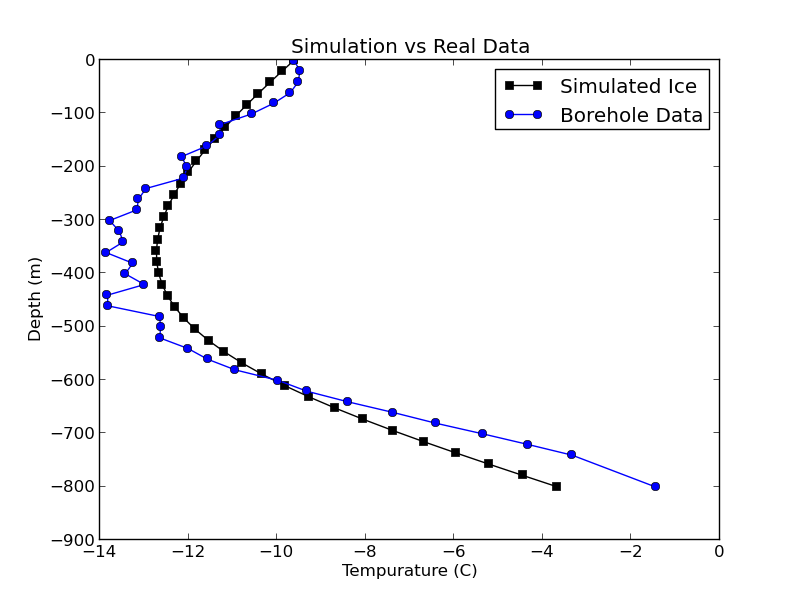
\includegraphics[width=0.48\textwidth]{../img/Simulation_vs_Real.png}
        \caption{Simulation curve compared to the actual temperature curve. $\dot{a} = 0.00355 ^m/_y$ and $u_b = 3.49 ^m/_y$}
    \end{figure}
    
    \begin{figure}[h!]
        \centering
        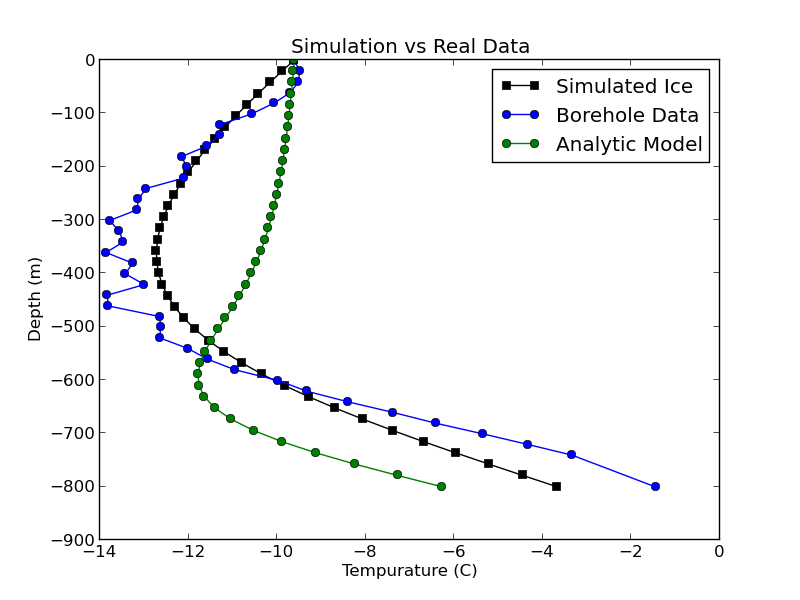
\includegraphics[width=0.48\textwidth]{../img/bad_analytic.png}
        \caption{Could not get the analytic solution to behave. $\dot{a} = 0.00355 ^m/_y$ and $u_b = 3.49 ^m/_y$}
    \end{figure}

    
    %%Analysis---------------------------------------------------------------------------
    \section{Analysis}
    Given the figures and the data. It appears that the implementation of the model is working correctly. An area of concern is top of the temperature curve. The data shows a slight increase in temperatures while the simulation does not. 

    %%Interpretation---------------------------------------------------------------------
    \section{Interpretation}
    The spike in temperature near the surface of the real glacier indicates that there is a process 
    that is trapping heat. This indicates that there is a limitation in the model that assumes heat cannot be trapped near the surface. Another possibility is that my implementation of the model contains an error that prevents the simulation from capturing the heat near the surface. 

    %%Critique---------------------------------------------------------------------------
    \section{Critique} 
    This is not really a critique, but there was a lot of variables to keep track of. Other than that the project was project was enjoyable. There is a single recommendation, post up the code showing what you plugged into your analytical function. i

    %%Bibliography-----------------------------------------------------------------------
    \begin{thebibliography}{1}
        \bibitem{3}\url{http://wiki.cs.umt.edu/classes/cs477/index.php/Ice\_Column\_Temperatures}
    \end{thebibliography} 

\end{document}
